\chapter{\label{chap:chap6}{Detailed Research Plan and Current Progress}}

\begin{figure}[b!]
\centering
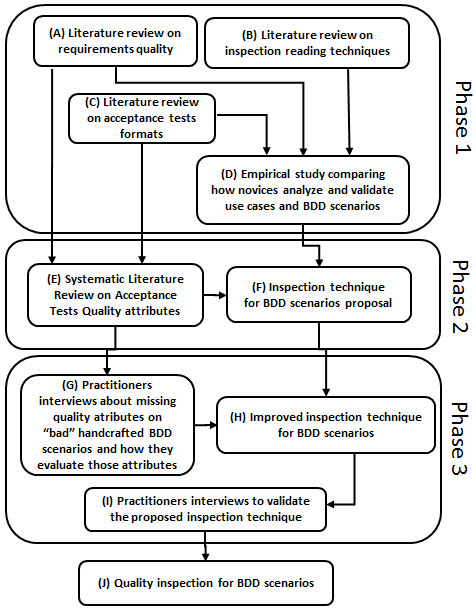
\includegraphics[scale=0.85]{images/Research-Plan-2}
\caption{Detailed research plan}
\label{fig:planning}
\end{figure}

As described in Chapter \ref{chap:chap3}, our goal is to create or adapt an inspection reading technique to assess the quality of BDD scenarios. To achieve that goal, we plan to combine the academic list of quality attributes that are useful to BDD scenarios with the practitioners opinions and our own background. The detailed research plan is summarized in Figure \ref{fig:planning}. 

\section{Current Progress}

%, when a draft of systematic literature review on the quality attributes of agile requirements was delivered as the final work on one of the post graduation curriculum classes. This systematic literature review is on protocol evaluation stage and we plan to start its execution as soon as this research plan is approved.

We have been performing a non-structured search on requirements quality, evaluation methods and known acceptance tests formats since June 2016 (represented in Figure \ref{fig:planning} \textbf{steps A, B and C} respectively). The requirements formats found on that effort were use cases, user stories and BDD and models. Since, user stories quality is already being evaluated by \cite{Lucassen_2015} and that our main goal was always to evaluate the quality of written BDD scenarios, we refined our goal and decided to undergo a full systematic literature review to acquire the quality attributes for acceptance tests. The rationale is that this concept can be represented by use cases, BDD scenarios or example tables as explained on Chapter \ref{chap:chap4}. Therefore, the attributes found on one of them should be useful to the others as well. We hope that the characteristics found could be translated to scenarios and help us to tackle the few existing information on what attributes a "good" scenario should shown. 

\ref{fig:planning} \textbf{step D} was planned as a moment to qualify our acquired knowledge by asking students to create use cases to a given set of software features and user stories and BDD scenarios to other set of features for a different application. After that data creation, the students were asked to validate their colleagues work using a list of quality attributes found on \cite{Babok_2015} (atomic, complete, consistent, concise, feasible, unambiguous, testable, prioritized and understandable) and \cite{Cohn_2004} (independent, negotiable, valuable, estimable, scalable, testable). The rationale of using both lists is that the first was meant to be used with traditional requirement formats only (like use cases) while the second is more suited for user stories. With the report of this study complete, the Phase 1 will be finished, as shown in Figure \ref{fig:planning}. 

\section{Additional Activities and Documents}

The report of the mentioned study will yield us an early version of a reading technique along with attributes, already empirically validated. However, we judge it would be wise to refine it with a systematic literature review on acceptance tests quality attributes and make sure there we used all the known state of the art knowledge. The systematic literature review is represented on \ref{fig:planning} \textbf{step E} already on Phase 2 and the proposed inspection technique is shown on \textbf{step F}.

Along with this Research Plan, the computer science graduate program at PUCRS asks for a seminar to evaluate the ongoing research before the full dissertation is delivered. On that occasion, we will show the results of the systematic literature review and how it refined our early draft reading technique obtained on the \textbf{step D}. We aim to ask for at least one BDD specialist review on it before presenting it to the board on the mentioned occasion. This should conclude the Phase 2 shown in Figure \ref{fig:planning}.

As we mentioned in prior chapters, there is no standard on what "good" scenarios are, but we have some examples of "bad" scenarios from \cite{Smart_2014}. One strategy that we devise to gather practitioners opinions is trough a series of interviews using "bad" scenarios. Using those examples, along with others taken from the empirical study and some handcrafted ones, we can ask practitioners the problems they see on them, the quality attributes they have missing and how they reached those conclusions. Those interviews are represented in Figure \ref{fig:planning} \textbf{step G}.

With both the quality characteristics and evaluation techniques taken from formal research and the ones taken from industry practitioners, we plan to conclude the reading technique that could assess the quality of BDD scenarios during the \textbf{step H} of Figure \ref{fig:planning}. Finally, it will need to be validated by industry and academic experts in order to establish its effectiveness and usefulness (\textbf{step I} in Figure \ref{fig:planning}).

The complete dissertation shall be delivered by the end of 2017. It will take the opinions of BDD practitioners to review and further refine the inspection reading technique and a second stage of practitioners opinions to validate it. This should conclude the Phase 3 shown in Figure \ref{fig:planning} and the \textbf{step J} in the same.

\section{Planned Timetable}

Table \ref{tbl:timetable} indicates an estimated timetable for the master's degree dissertation.

\begin{table}[!h]
\centering
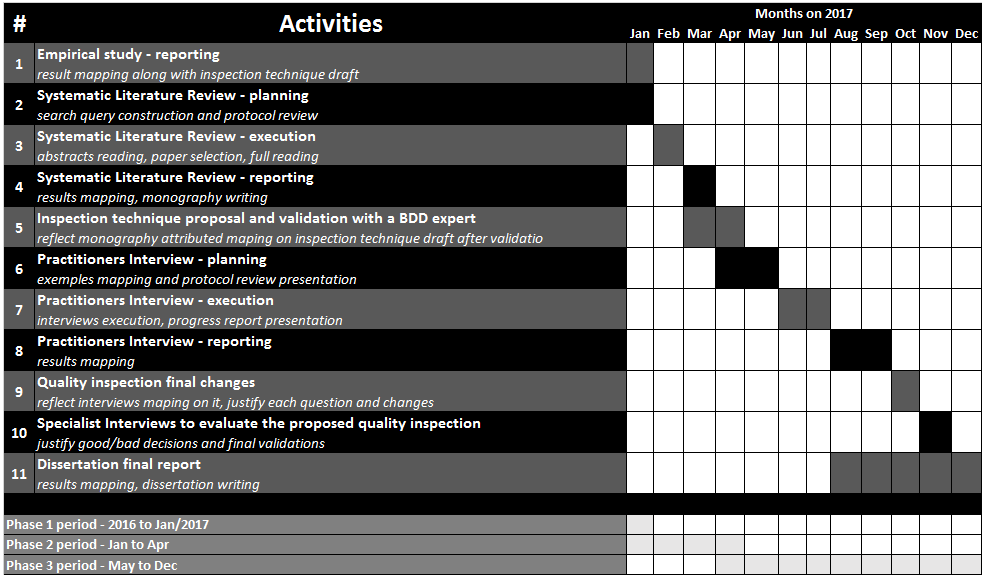
\includegraphics[scale=0.65]{images/Planning-Table}
\caption{Detailed research plan timetable}
\label{tbl:timetable}
\end{table}
